\documentclass{article}
\usepackage{graphicx}
\title{HÜ1: Latex-Tabelle mit skalierten und rotierten Bildern}
\author{Ogulcan Seyran}
\date{25.04.2022}
\begin{document}
	\maketitle
	\begin{center}
		\begin{tabular}{ |c |c |c| }
			\hline
			Normal & Skaliert & Rotiert \\
			\hline
			
\includegraphics[scale=0.3]{cow.png} & 
\includegraphics[scale=0.15]{cow.png} & 
\includegraphics[scale=0.3,angle=45]{cow.png} \\ 
			\hline
			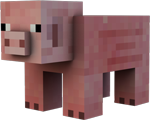
\includegraphics[scale=0.3]{pig.png} & 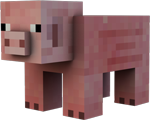
\includegraphics[scale=0.15]{pig.png} & 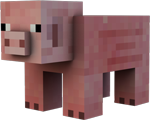
\includegraphics[scale=0.3,angle=15]{pig.png} \\ 
			\hline
			
\includegraphics[scale=0.3]{chicken.png} & 
\includegraphics[scale=0.15]{chicken.png} & 
\includegraphics[scale=0.3,angle=90]{chicken.png} \\ 
			\hline
		\end{tabular}
	\end{center}
\end{document}